\section{Implementación}
\subsection{Arquitectura General}
La implementación se dividió en varios módulos con responsabilidades bien definidas, siguiendo principios de diseño orientado a objetos.
El sistema está compuesto por tres componentes principales:

\begin{enumerate}
    \item \textbf{Cliente (upload.py / download.py):} Aplicaciones CLI independientes
    \item \textbf{Servidor (start-server.py):} Servidor concurrente multi-thread
    \item \textbf{Librería RDT (lib/):} Módulos compartidos para el protocolo
\end{enumerate}

\subsection{Estructura de paquetes}
Todos los paquetes siguen una estructura de header fijo de 14 bytes seguido de un payload variable.

\begin{table}[H]
\centering
\begin{tabular}{@{}lll@{}}
\toprule
\textbf{Campo}        & \textbf{Tamaño} & \textbf{Descripción} \\ \midrule
\texttt{seq\_num}     & 1 byte  & Número de secuencia (0-255, con wrap-around) \\
\texttt{checksum}     & 1 byte  & Suma de verificación para detección de errores \\
\texttt{ack\_num}     & 1 byte  & Número de ACK (usado en paquetes ACK) \\
\texttt{payload\_length} & 4 bytes & Longitud del payload en bytes \\
\texttt{file\_size}   & 4 bytes & Tamaño total del archivo (solo en INIT) \\
\texttt{packet\_type} & 1 byte  & Tipo de paquete (ver tabla siguiente) \\
\texttt{protocol}     & 1 byte  & Protocolo utilizado (1=Stop\&Wait, 2=Selective Repeat) \\
\texttt{session\_id}  & 1 byte  & Identificador de sesión (1-255) \\ \bottomrule
\end{tabular}
\caption{Campos del Header (14 bytes)}
\end{table}

\subsection{Tipos de paquetes}
En el protocolo implementado, cada paquete tiene un tipo específico que determina su función dentro de la transferencia de archivos. A continuación se describen los tipos de paquetes utilizados y su propósito principal:

\begin{itemize}
    \item \textbf{DATA (1)}: Transferencia de datos, contiene los fragmentos del archivo.
    \item \textbf{ACK (2)}: Acknowledgment de paquetes DATA recibidos correctamente.
    \item \textbf{UPLOAD\_INIT (3)}: Inicia una sesión de subida (upload) de archivo.
    \item \textbf{DOWNLOAD\_INIT (4)}: Inicia una sesión de descarga (download) de archivo.
    \item \textbf{ACCEPT (5)}: Acepta la transferencia en respuesta a un paquete INIT.
    \item \textbf{ACCEPT\_ACK (6)}: Confirma la finalización del handshake.
    \item \textbf{FIN (7)}: Indica la finalización de la transferencia de datos.
    \item \textbf{FIN\_ACK (8)}: Confirma la finalización de la sesión.
    \item \textbf{ERROR (9)}: Mensaje de error, enviado por el servidor ante problemas o rechazos.
\end{itemize}

\begin{table}[H]

\label{tab:packet_types}
\renewcommand{\arraystretch}{1.2}
\begin{tabularx}{\textwidth}{|p{2.5cm}|p{3cm}|X|X|}
\hline
\textbf{Tipo} & \textbf{Dirección} & \textbf{Payload} & \textbf{Campos Relevantes} \\ \hline

\textbf{UPLOAD
\_INIT (3)}
& Cliente $\rightarrow$ Servidor
& Nombre del archivo (UTF-8)
& \texttt{file\_size} (bytes), \texttt{protocol}, \texttt{session\_id=0} \\ \hline

\textbf{DOWNLOAD
\_INIT (4)}
& Cliente $\rightarrow$ Servidor
& Nombre del archivo (UTF-8)
& \texttt{file\_size=0}, \texttt{protocol}, \texttt{session\_id=0} \\ \hline

\textbf{ACCEPT (5)}
& Servidor $\rightarrow$ Cliente
& Puerto dedicado en ASCII (ej: ``52341'') o vacío
& \texttt{session\_id} (1–255 asignado) \\ \hline

\textbf{ACCEPT
\_ACK (6)}
& Cliente $\rightarrow$ Servidor
& Vacío
& \texttt{session\_id}, \texttt{ack\_num=0} \\ \hline

\textbf{DATA (1)}
& Bidireccional
& Fragmento de archivo (hasta 4096 bytes)
& \texttt{seq\_num}, \texttt{session\_id}, \texttt{payload\_length} \\ \hline

\textbf{ACK (2)}
& Receptor $\rightarrow$ Emisor
& Vacío
& \texttt{ack\_num}, \texttt{session\_id} \\ \hline

\textbf{FIN (7)}
& Emisor $\rightarrow$ Receptor
& Vacío
& \texttt{session\_id} \\ \hline

\textbf{FIN\_ACK (8)}
& Receptor $\rightarrow$ Emisor
& Vacío
& \texttt{session\_id} \\ \hline

\textbf{ERROR (9)}
& Servidor $\rightarrow$ Cliente
& Mensaje de error en UTF-8
& Texto descriptivo (ej: ``File not found'') \\ \hline

\end{tabularx}
\centering
\caption{Tipos de Paquetes del Protocolo}
\end{table}

\subsection{Flujos del Protocolo}
\subsubsection{Handshake (upload)}

\begin{figure}[H]
    \centering
    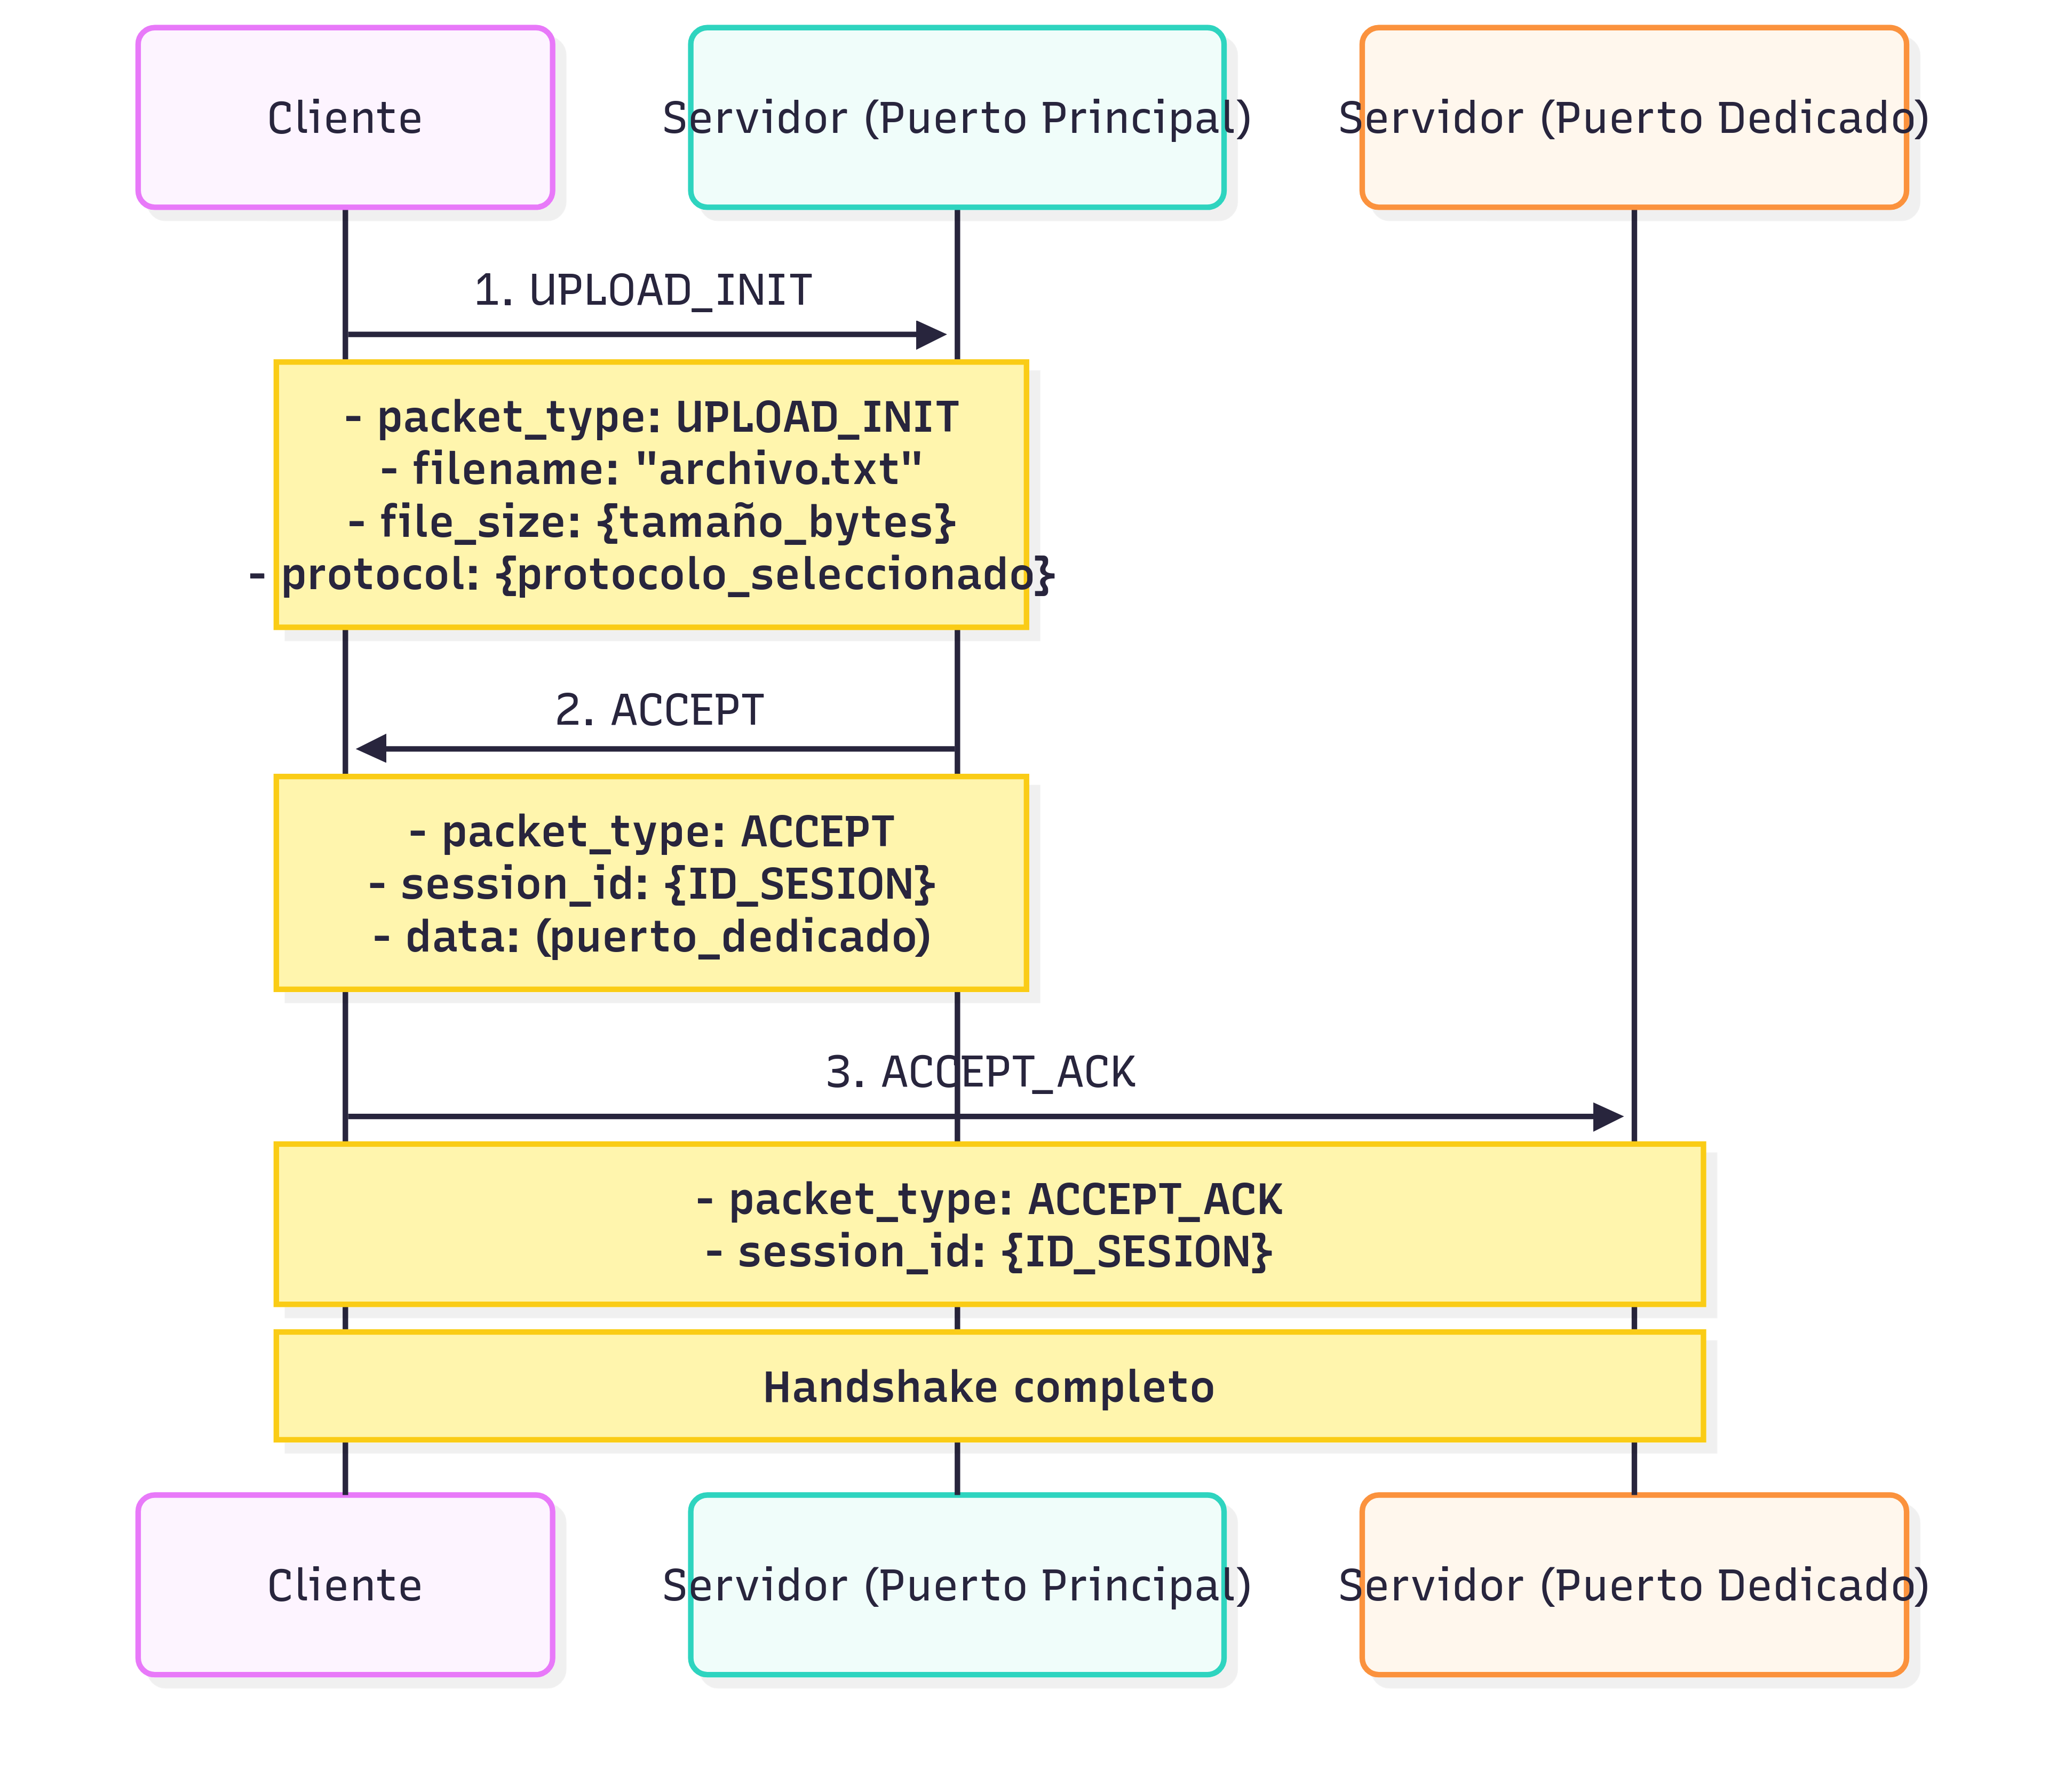
\includegraphics[width=1\linewidth]{images/UPLOAD_HANDSHAKE}
    \caption{Handshake inicial para subida de archivo}
    \label{fig:upload_handshake}
\end{figure}

\subsubsection{Handshake (download)}

\begin{figure}[H]
    \centering
    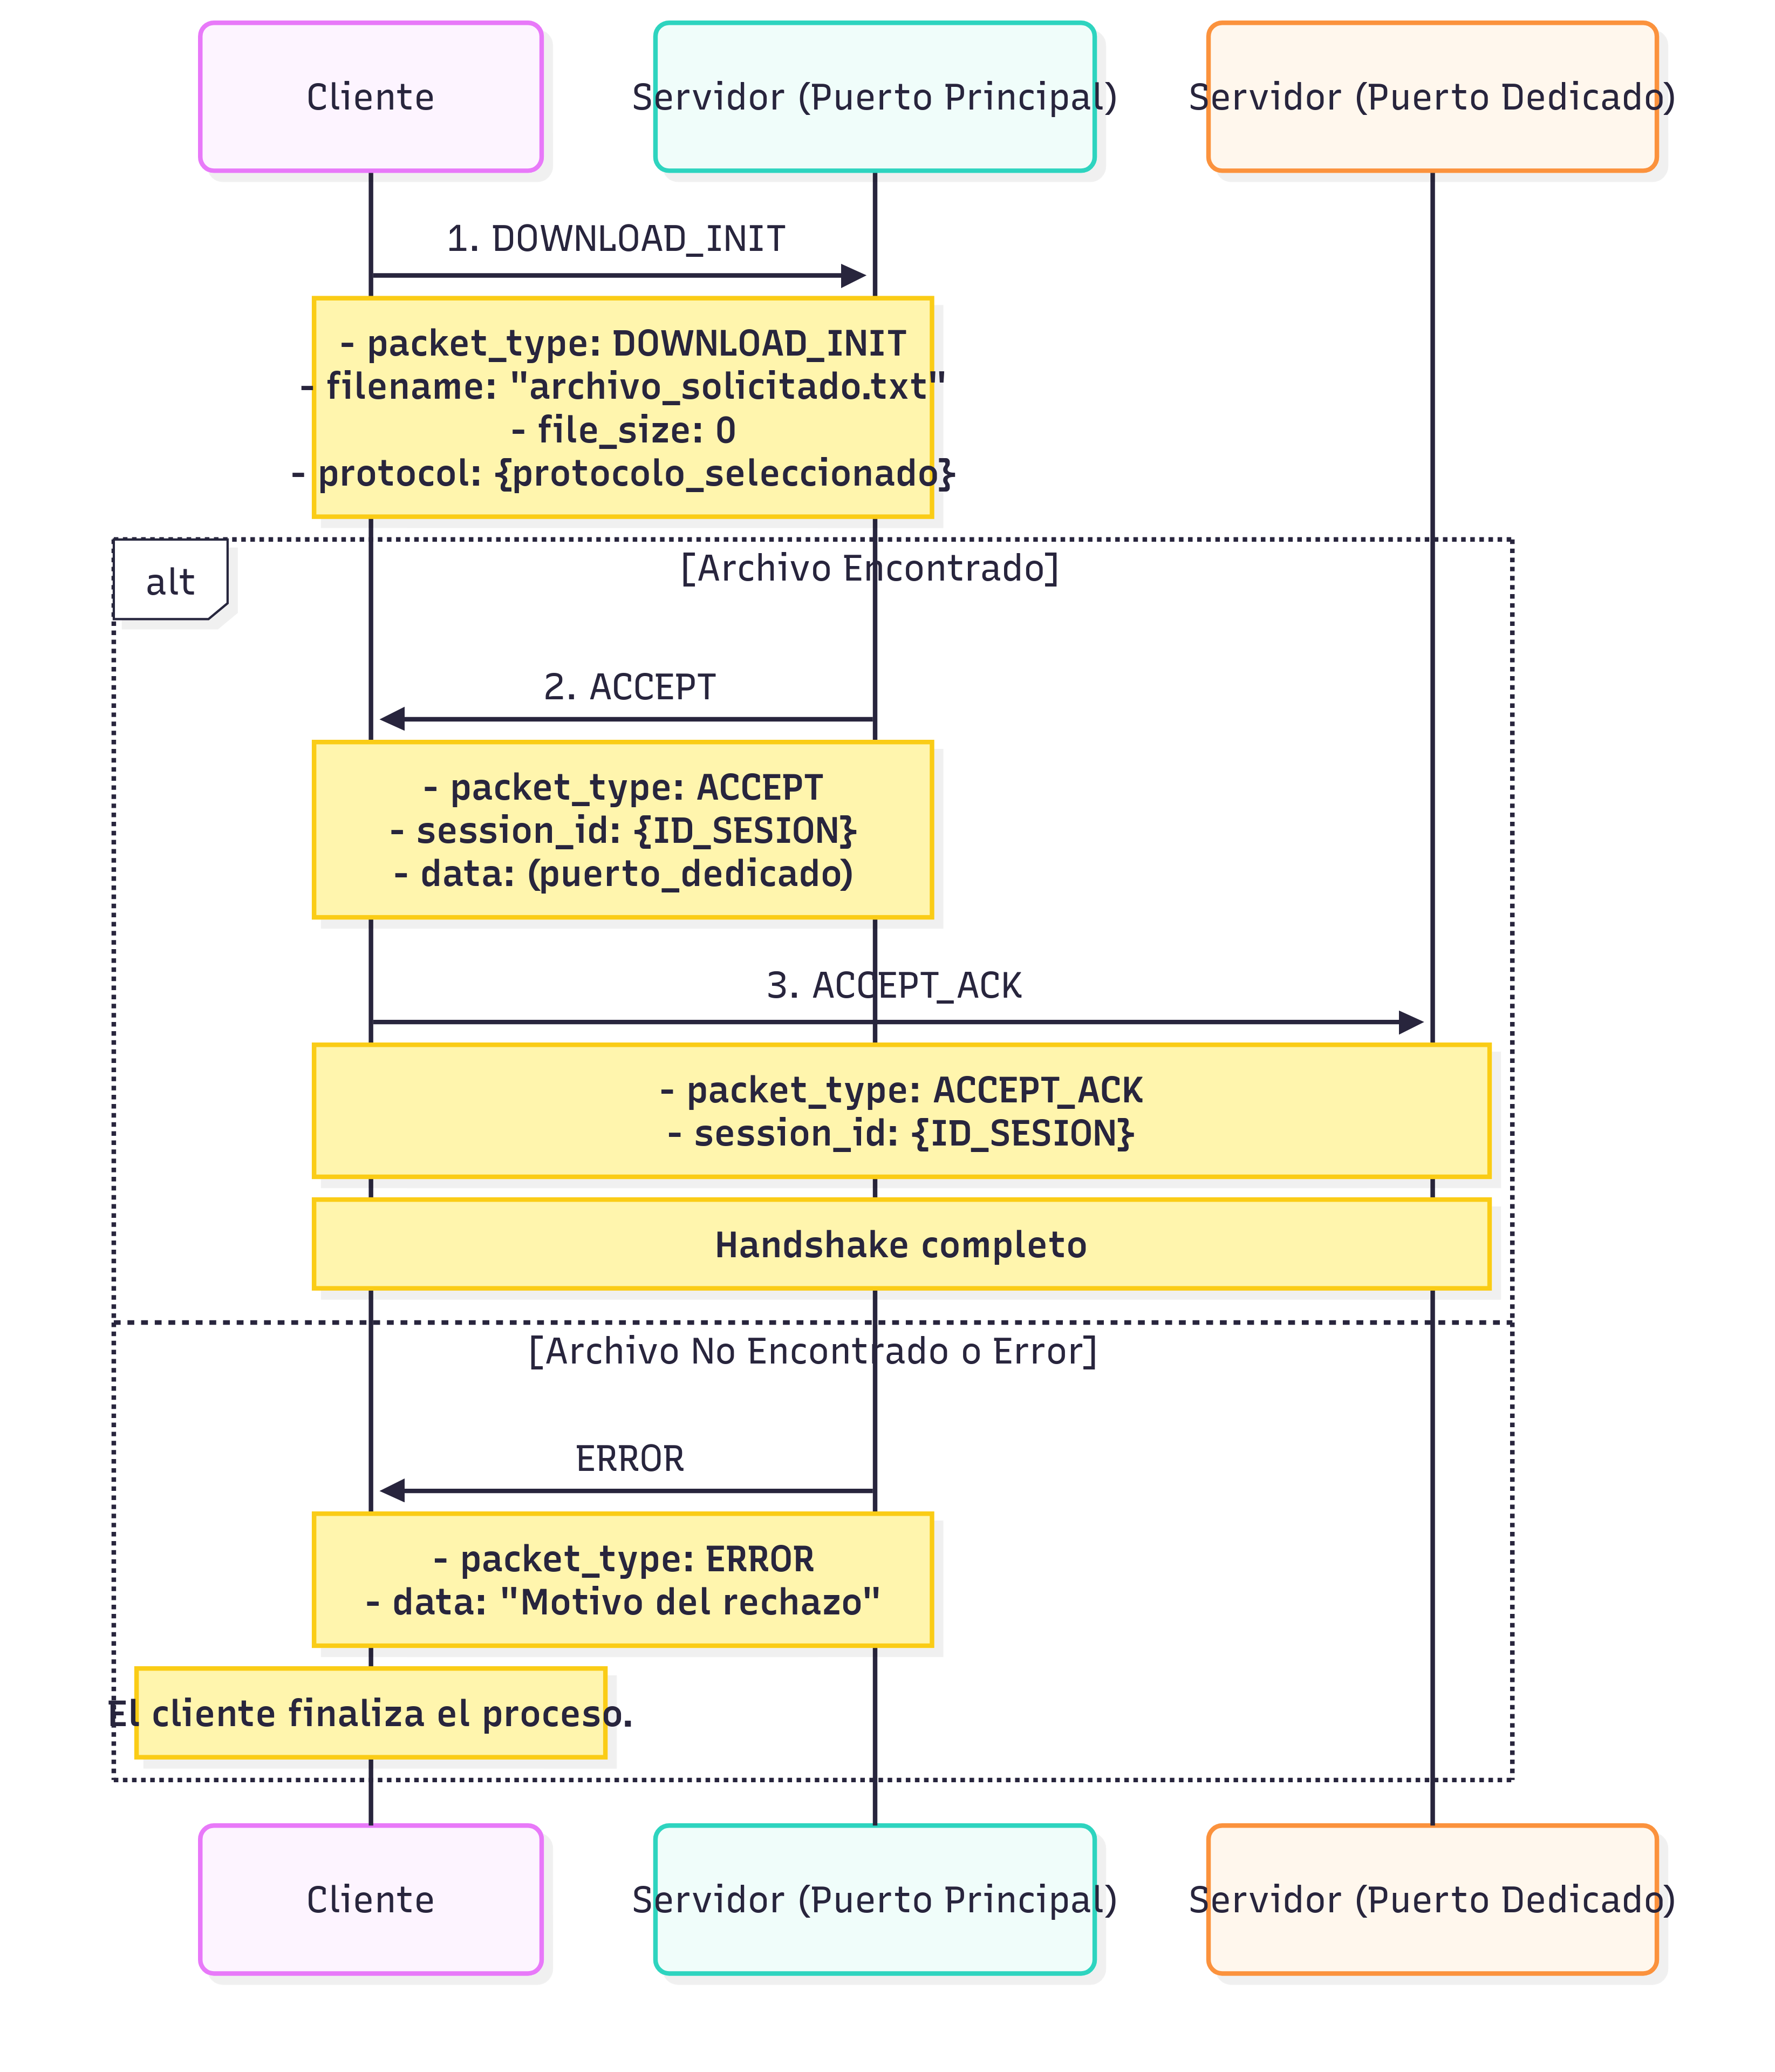
\includegraphics[width=1\linewidth]{images/DOWNLOAD_HANDSHAKE}
    \caption{Handshake inicial para descarga de archivo}
    \label{fig:download_handshake}
\end{figure}

\subsubsection{Cierre de conexion}

\begin{figure}[H]
    \centering
    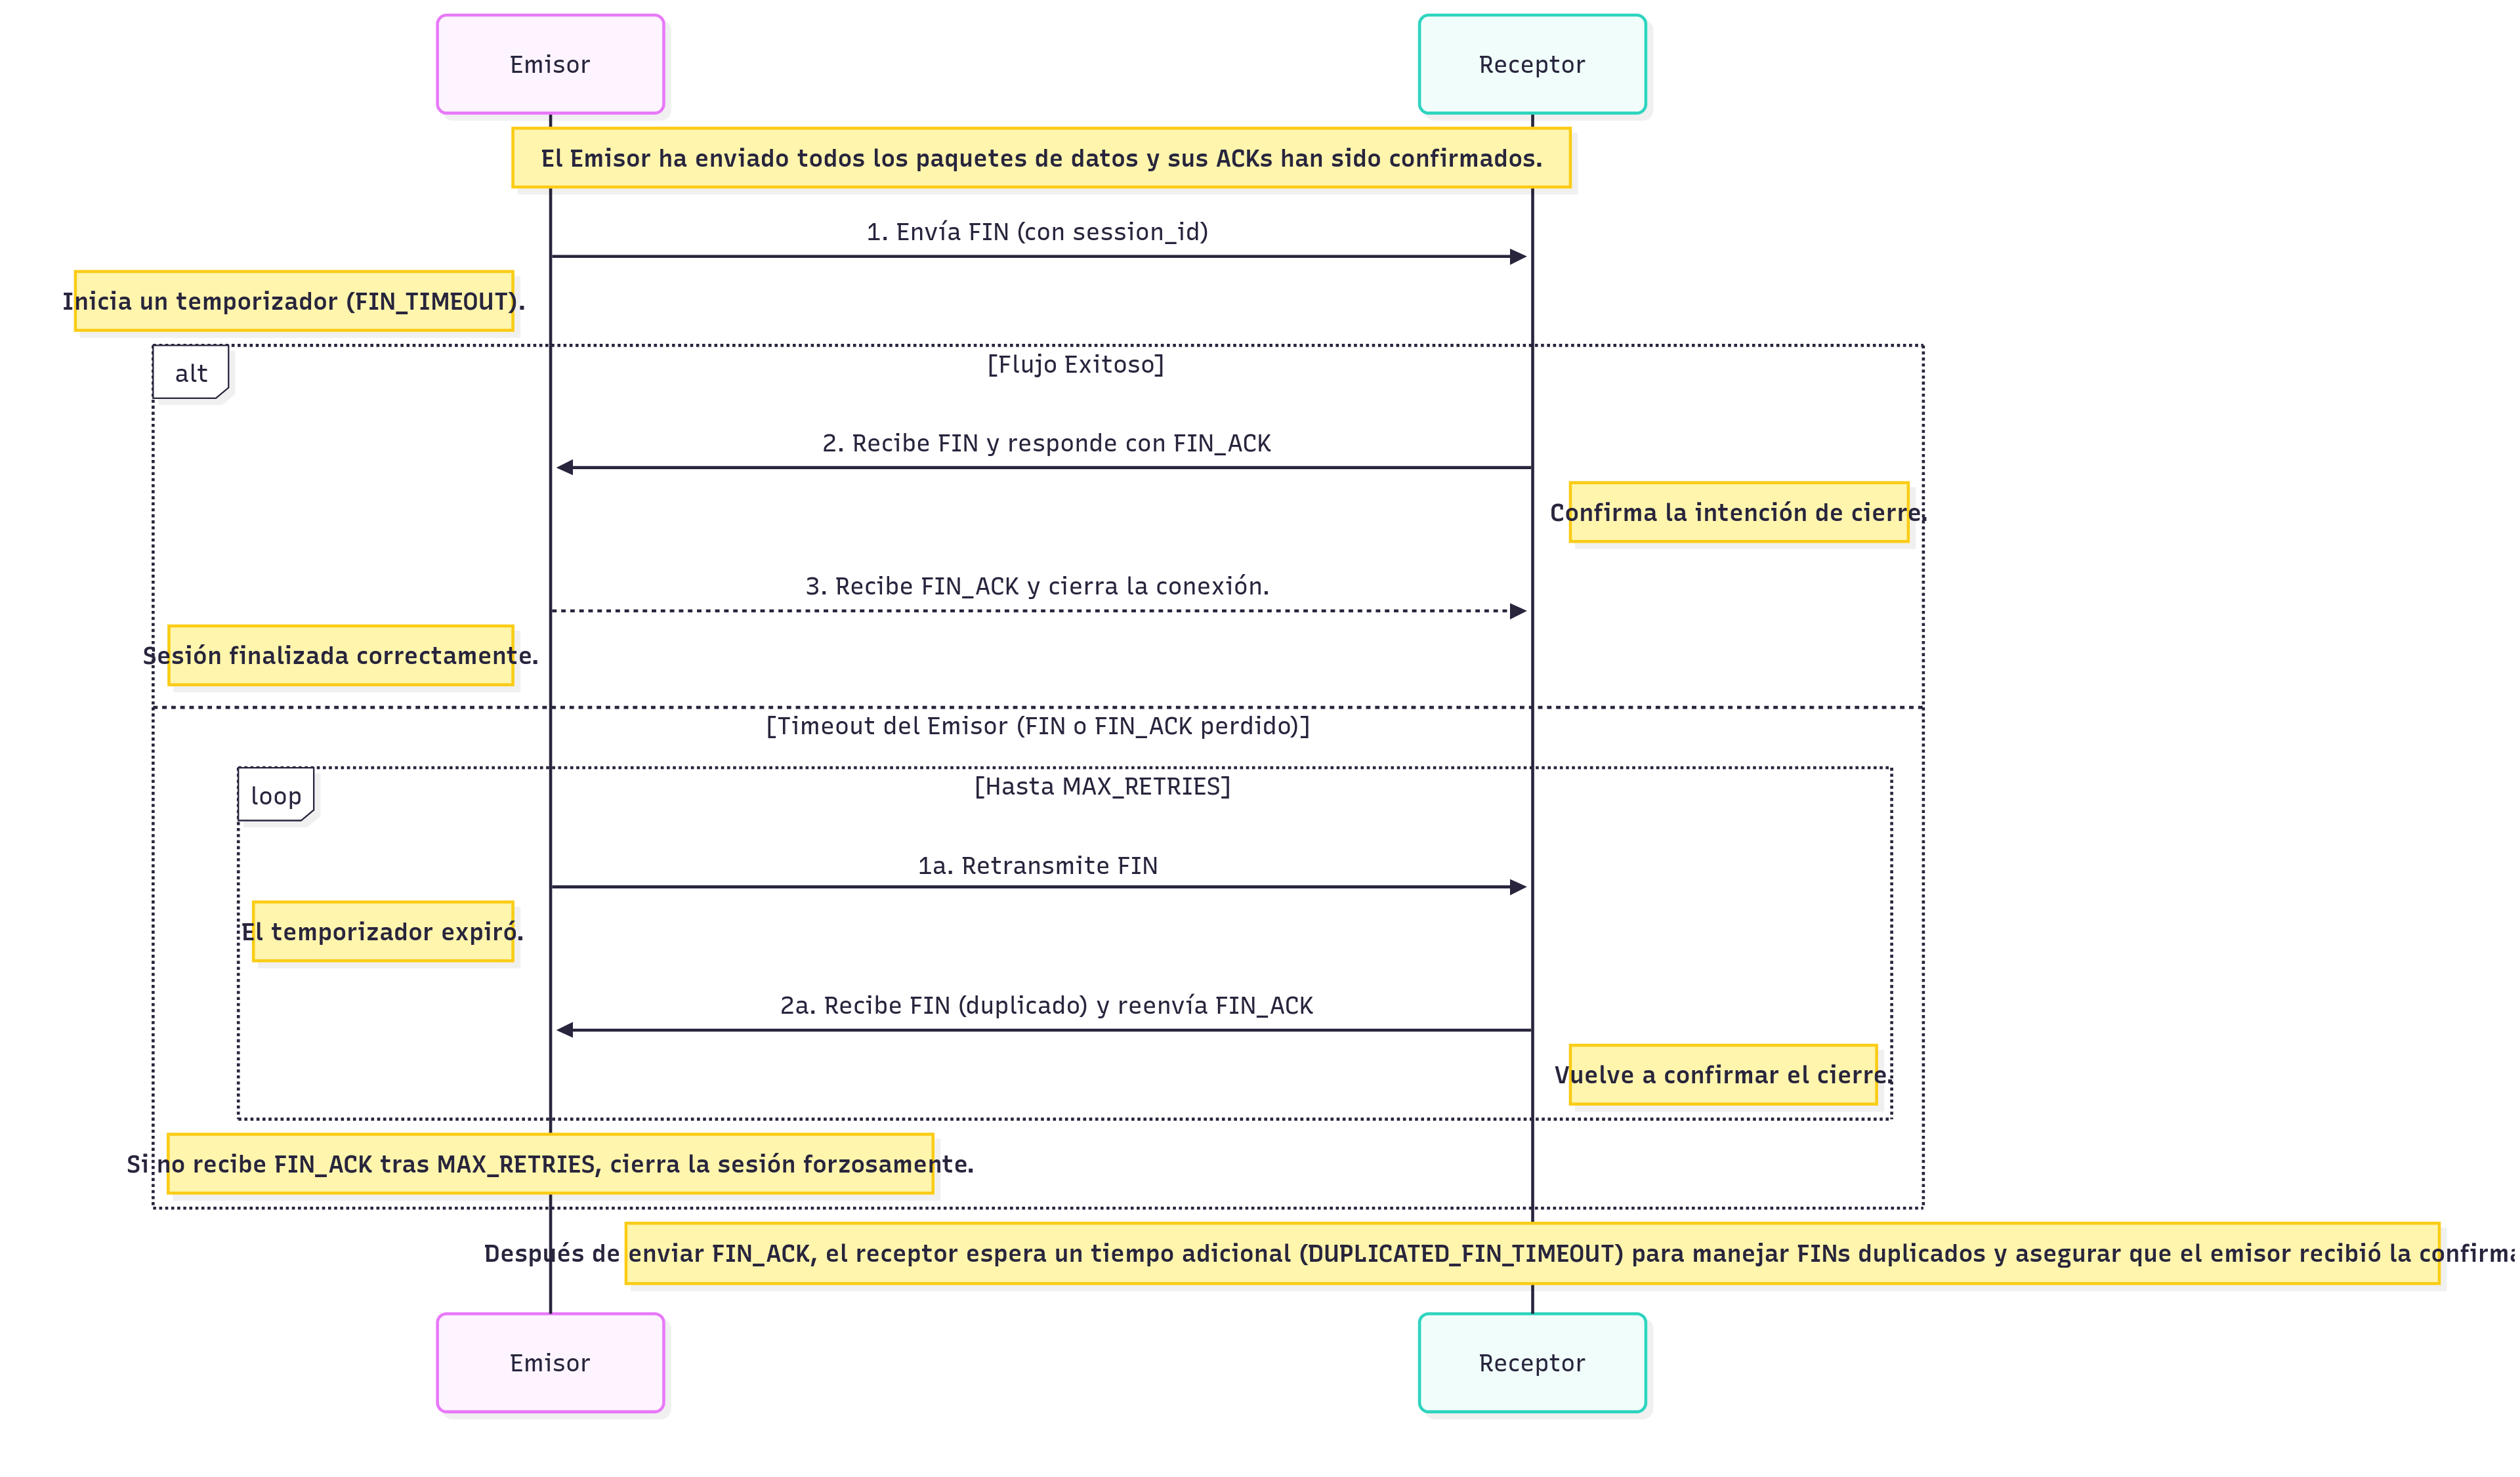
\includegraphics[width=1\linewidth]{images/FIN}
    \caption{Subida / Descarga de archivo con Selective Repeat}
    \label{fig:fin_transfer}
\end{figure}

\subsubsection{Subida / Descarga de archivo}
En el caso de una subida de archivo, el emisor es el Cliente y el receptor el Servidor. En el caso de una descarga, el emisor es el Servidor y el receptor el Cliente. El flujo de envio de paquetes DATA es el mismo para ambos casos.
\begin{figure}[H]
    \centering
    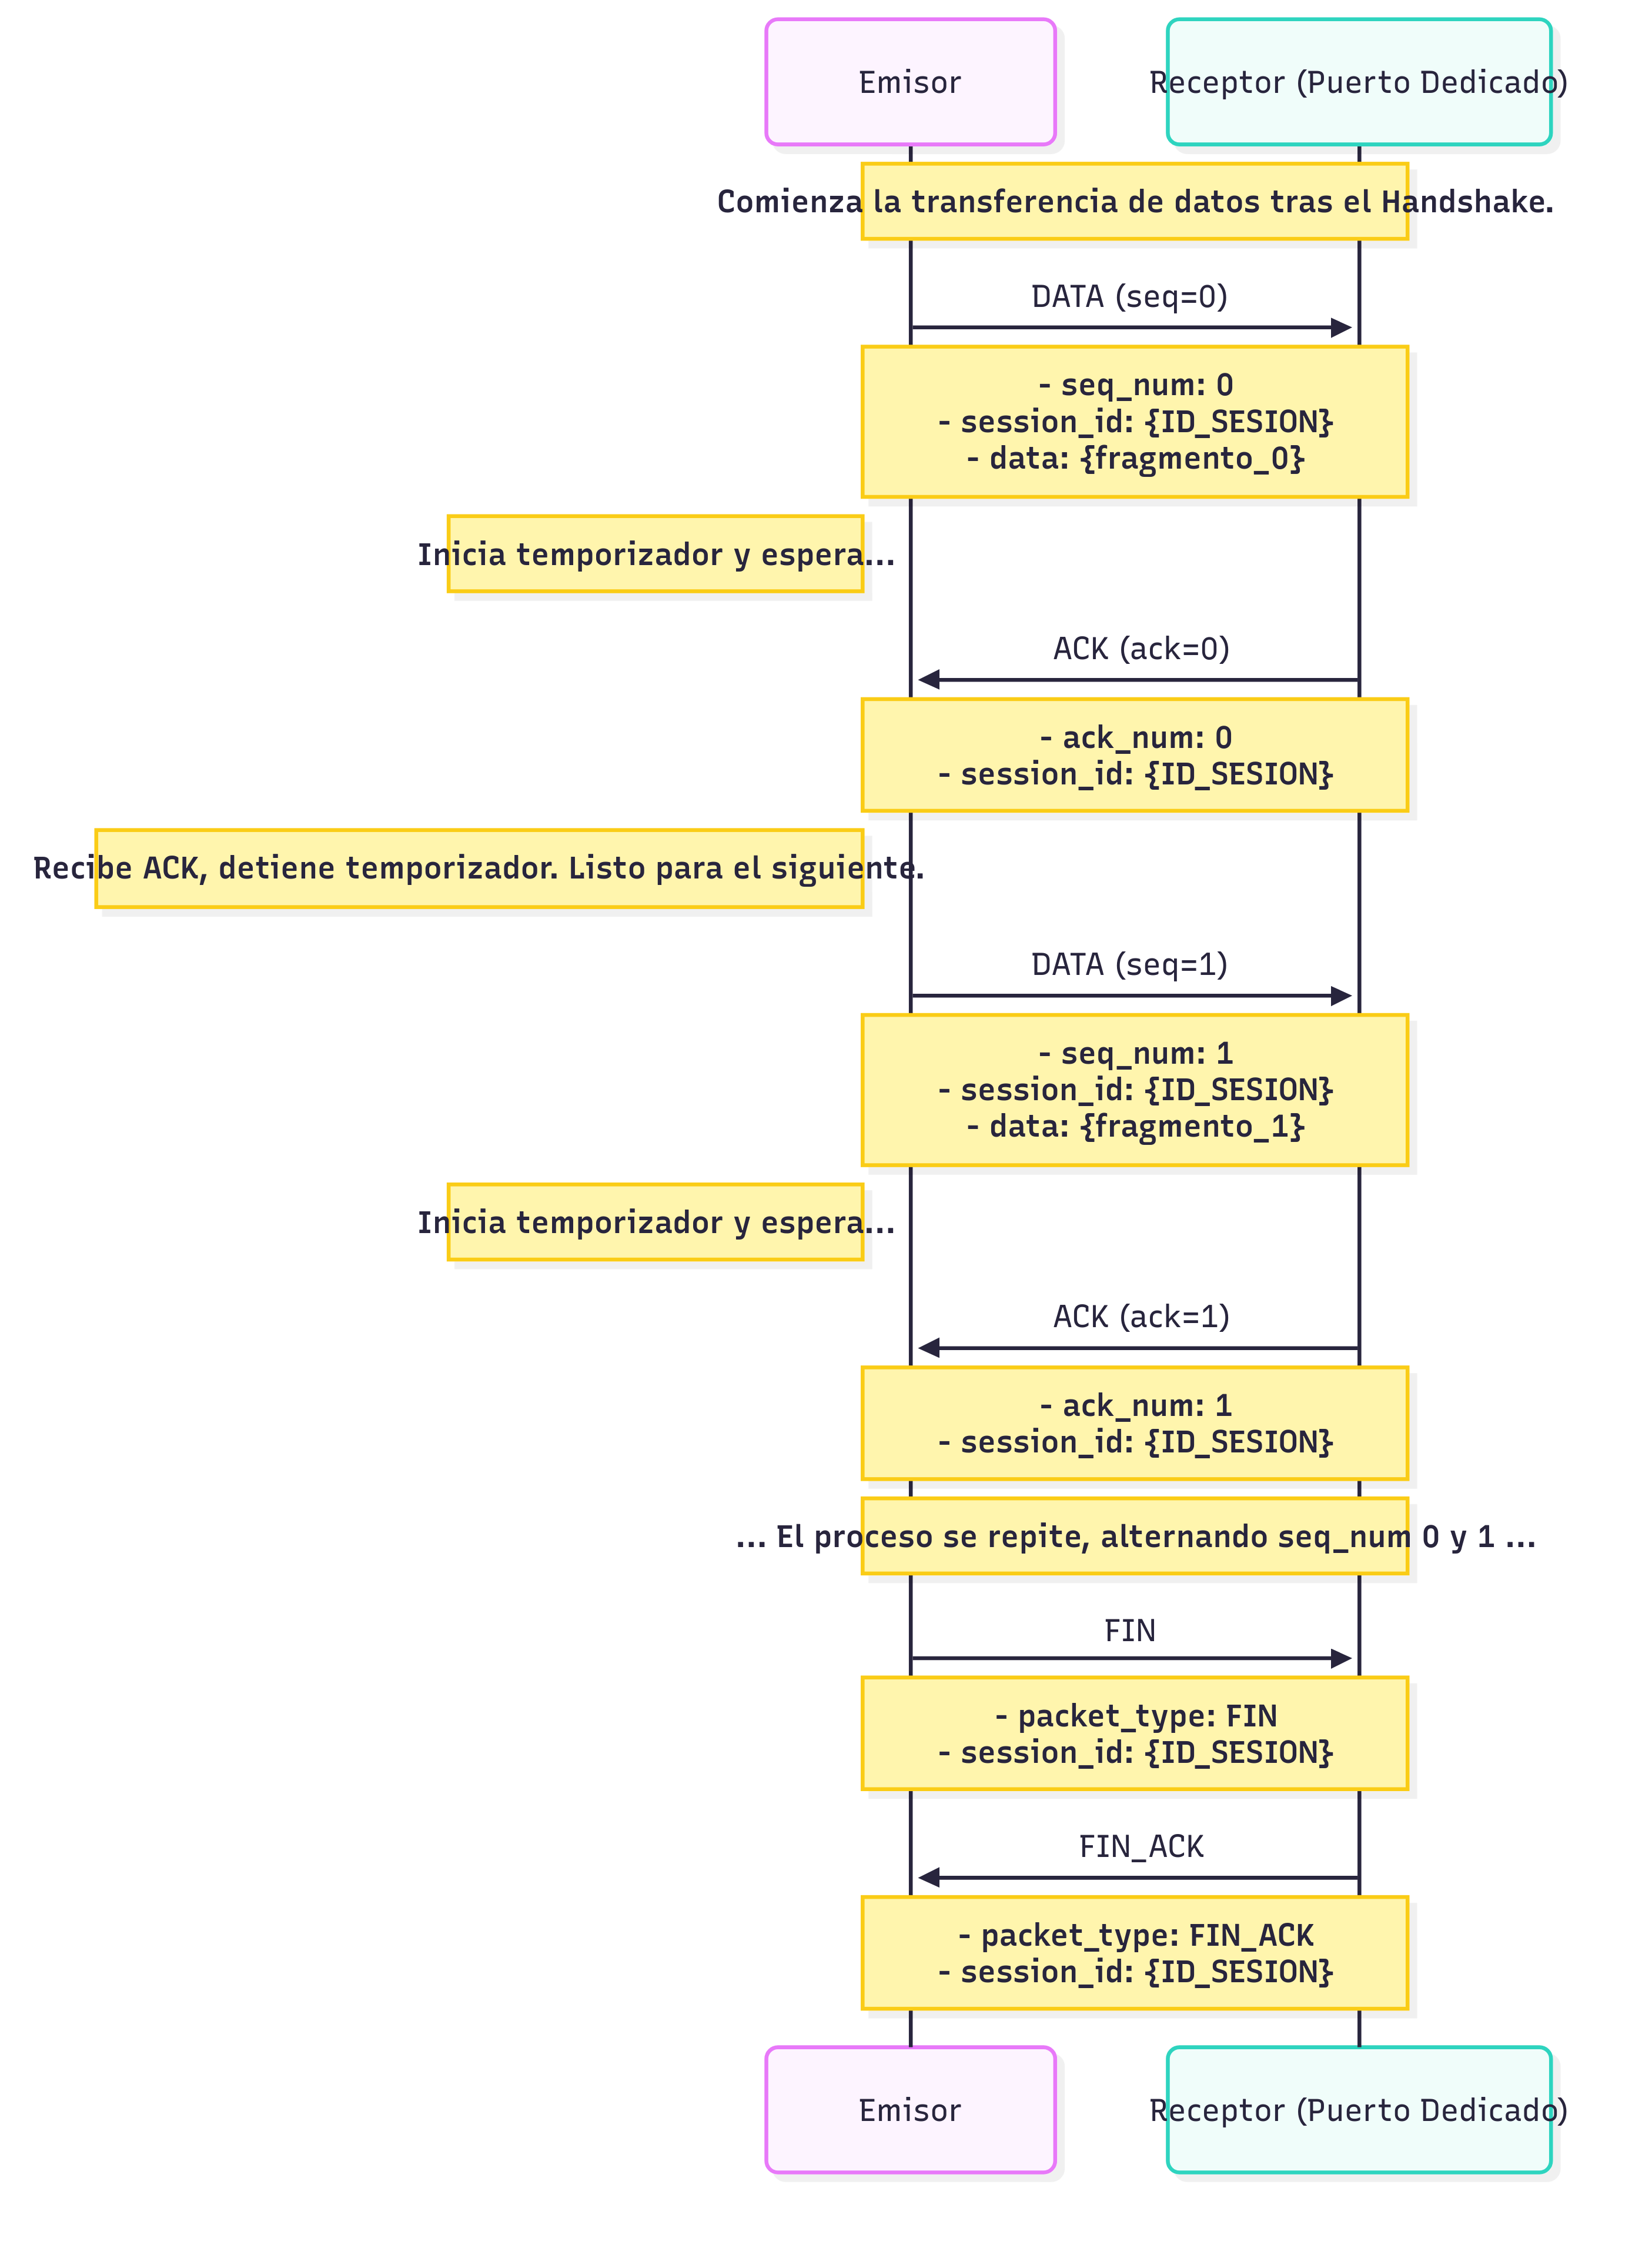
\includegraphics[height=0.8\textheight]{images/UPLOAD_DOWNLOAD}
    \caption{Subida / Descarga de archivo con Stop \& Wait}
    \label{fig:upload_download_sw}
\end{figure}

\begin{figure}[H]
    \centering
    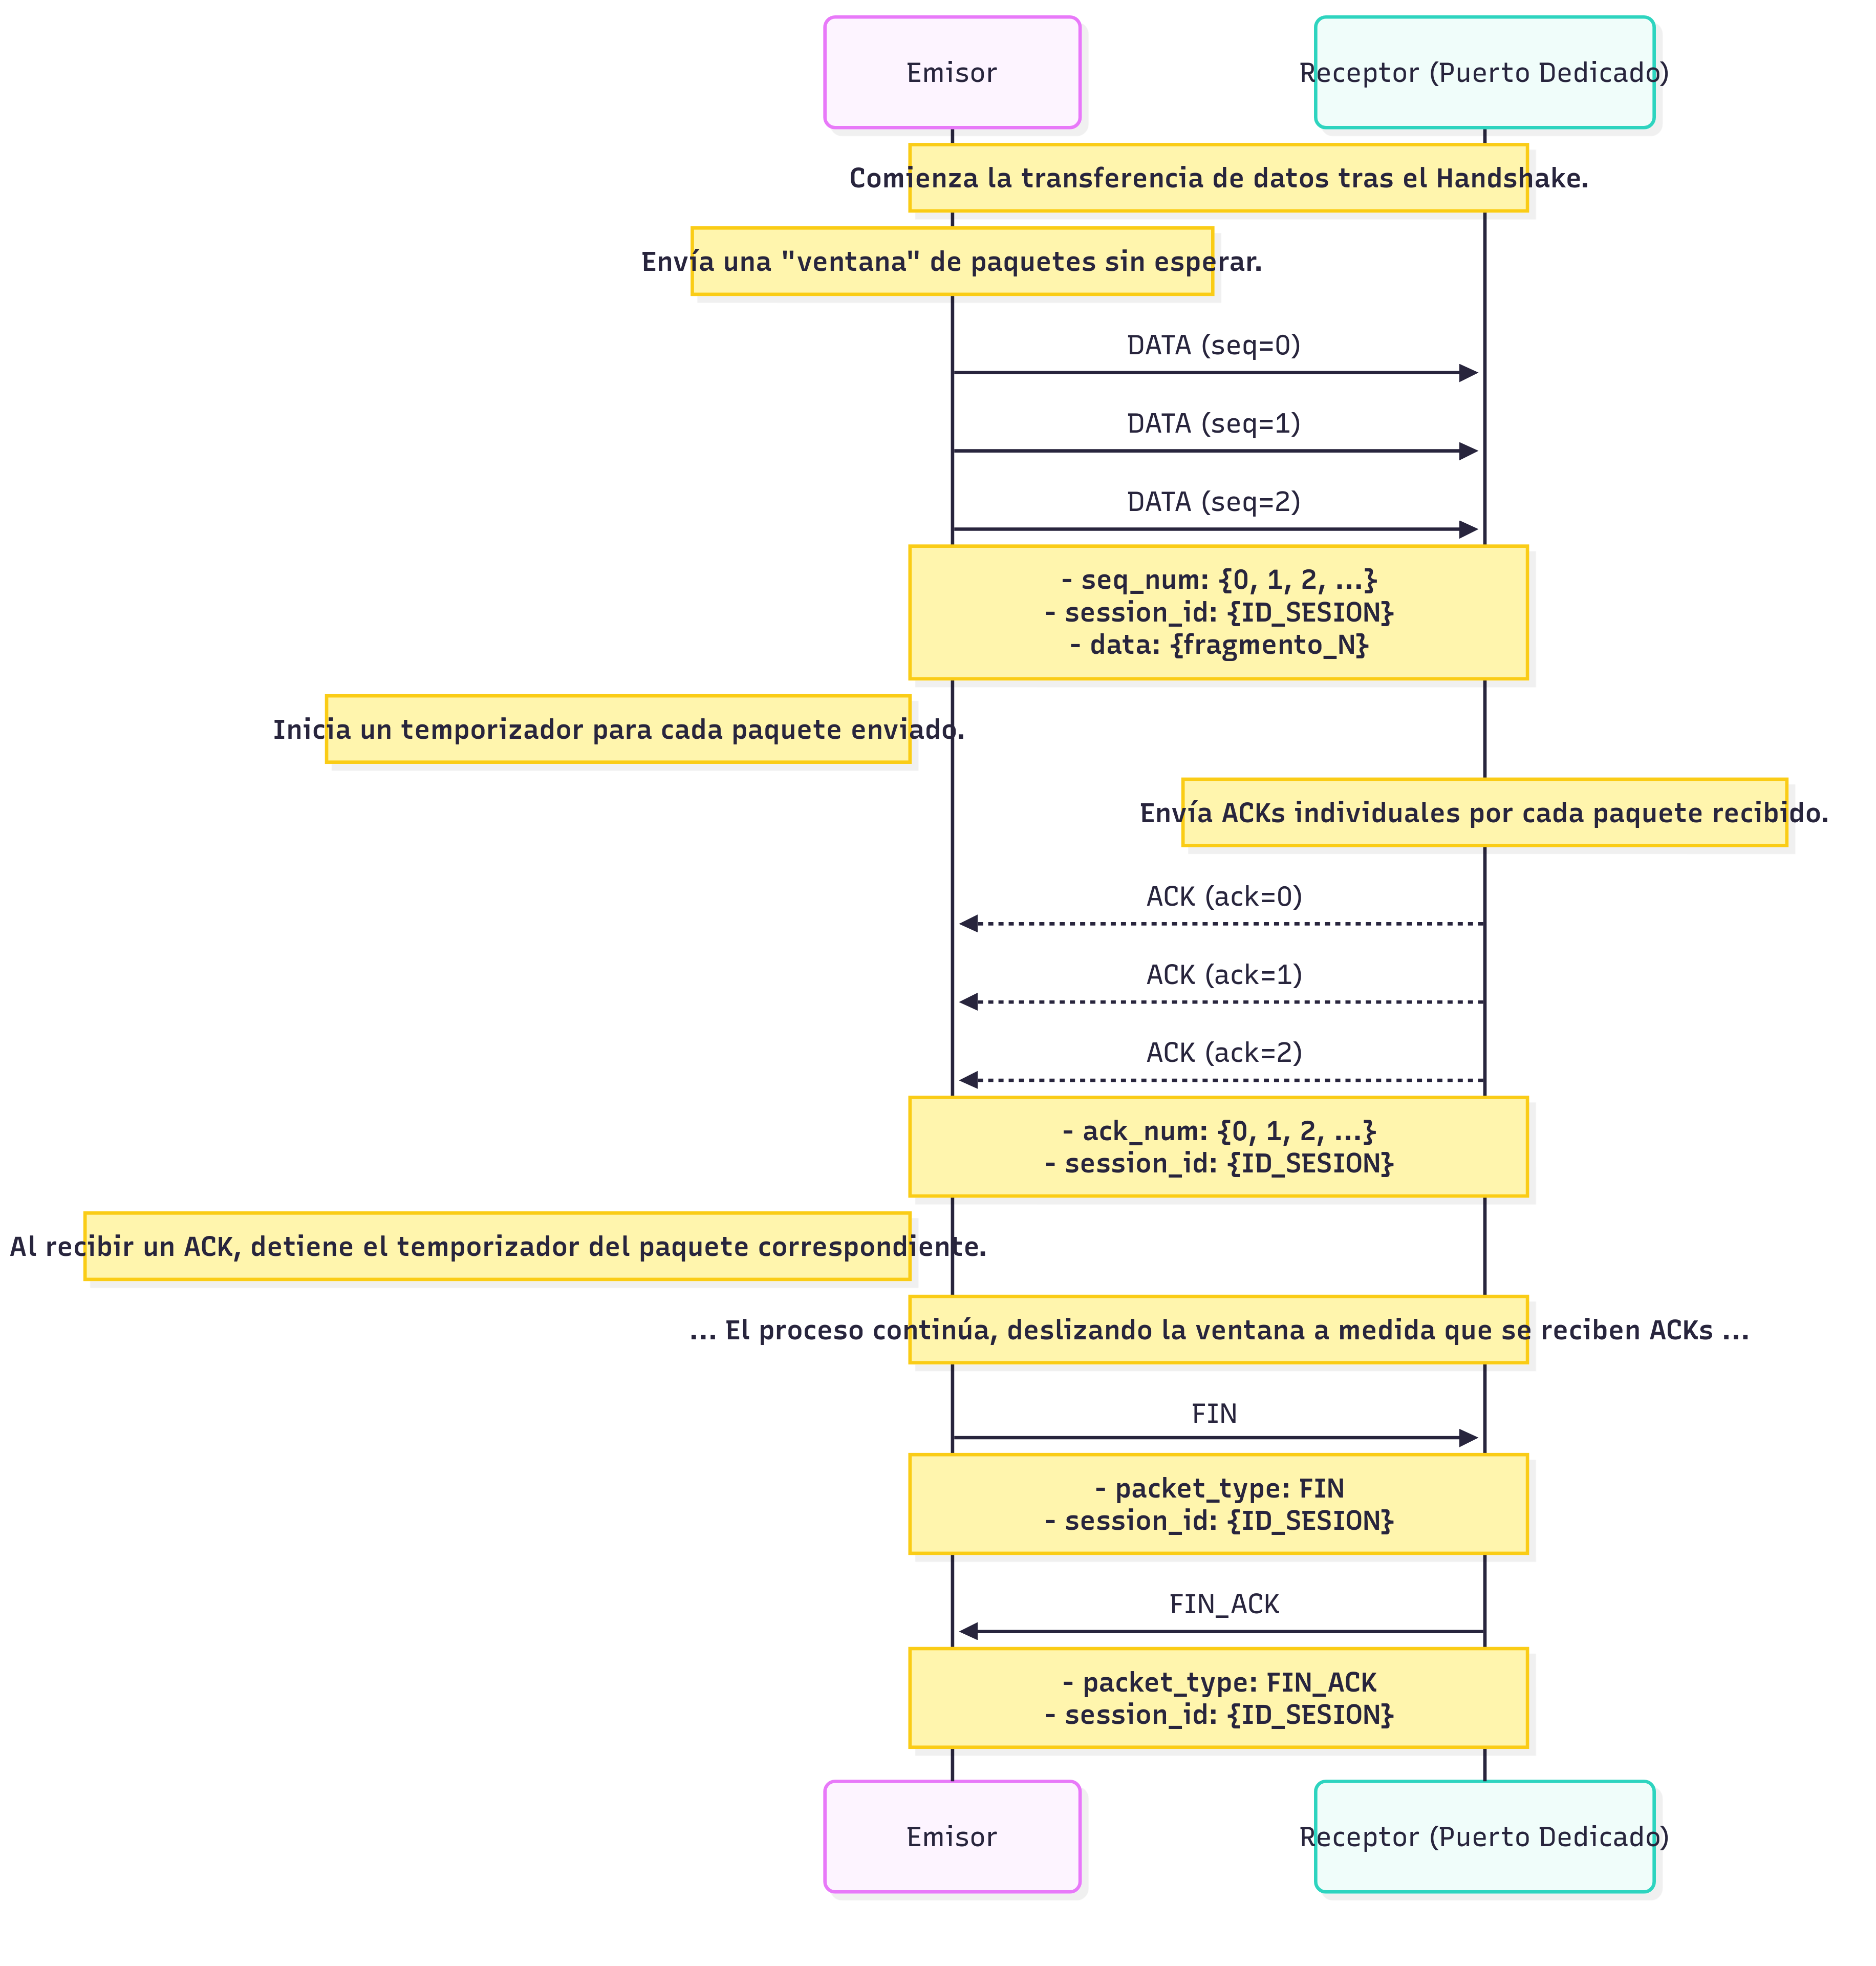
\includegraphics[height=0.8\textheight]{images/UPLOAD_DOWNLOAD_SR}
    \caption{Subida / Descarga de archivo con Selective Repeat}
    \label{fig:upload_download_sr}
\end{figure}

\subsection{Manejo de errores}
El sistema implementa múltiples capas de manejo de errores:

\begin{enumerate} [label=\roman*. , leftmargin=2cm]
    \item \textbf{Validación de Checksums:}\\
    Cada paquete incluye un checksum simple (suma de los bytes del payload, metadatos y encabezado). El receptor valida la integridad recalculando el checksum y comparándolo. En caso de que el paquete este corrupto, se descarta y no se envía confirmación, forzando retransmisión por timeout.

    \item \textbf{Timeouts y Retransmisiones:}\\
    Cada emisor asocia un temporizador a los paquetes enviados, si no se recibe el ACK correspondiente dentro del tiempo configurado, el paquete se retransmite asegurando la entrega aún bajo pérdidas del 10\% simuladas en Mininet.

    \item \textbf{Control de duplicados:}\\
    Stop \& Wait: gracias al uso de números de secuencia binarios (0/1), el receptor distingue duplicados fácilmente.\\
    Selective Repeat: mantiene una ventana deslizante con buffer y descarta paquetes ya recibidos fuera de ventana.

    \item \textbf{Manejo de paquetes fuera de orden:}\\
    Stop \& Wait: no admite desorden, cualquier paquete inesperado se ignora.\\
    Selective Repeat: almacena los paquetes válidos recibidos fuera de orden en el buffer, enviando igualmente ACKs, hasta que pueda reconstruir el flujo completo.

    \item \textbf{Mensajes de control específicos:}\\
    ERROR: permite rechazar solicitudes inválidas (por ejemplo, archivo inexistente o en uso) \\
    FIN / FIN-ACK: asegura el cierre limpio de la sesión, evitando que un corte abrupto deje la conexión en estado inconsistente.

\end{enumerate}
A continuación, se presentan diagramas de secuencia que ilustran lo explicado en algunos de los items anteriores:

\begin{figure}[H]
    \centering
    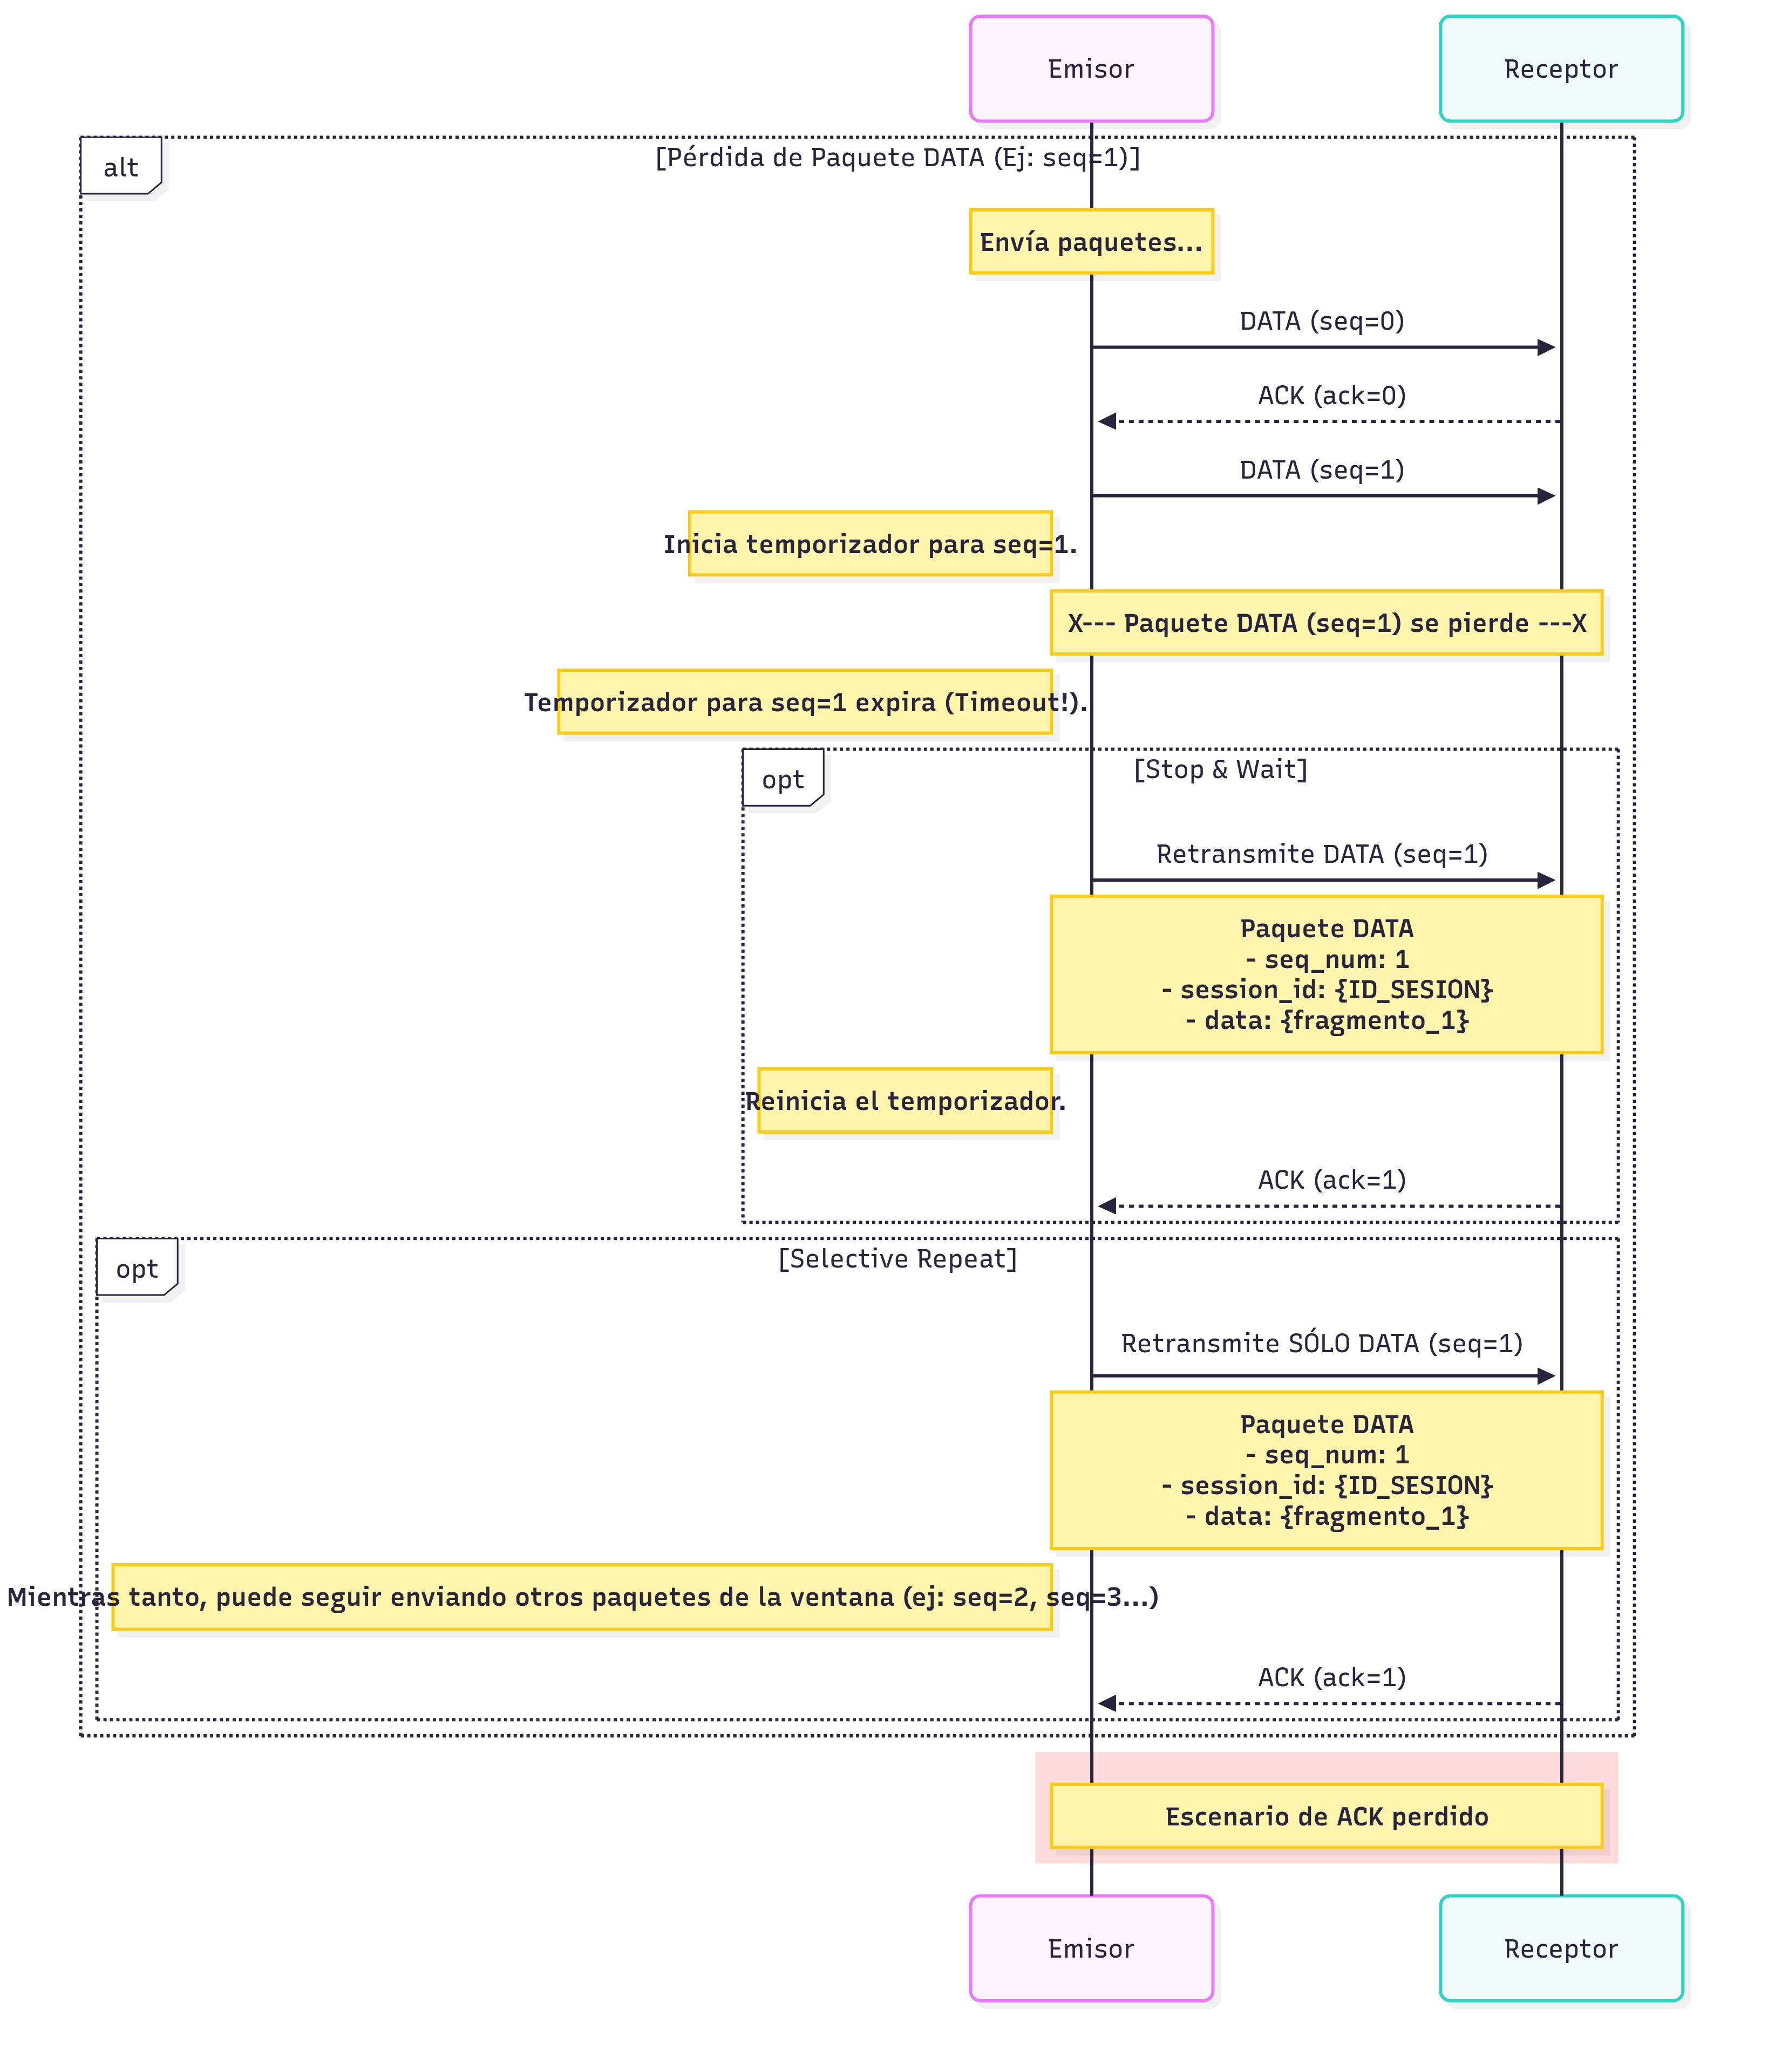
\includegraphics[width=1\linewidth]{images/RETRANSMISION}
    \caption{Retramision de paquetes por timeout.}
    \label{fig:retransmision}
\end{figure}

\begin{figure}[H]
    \centering
    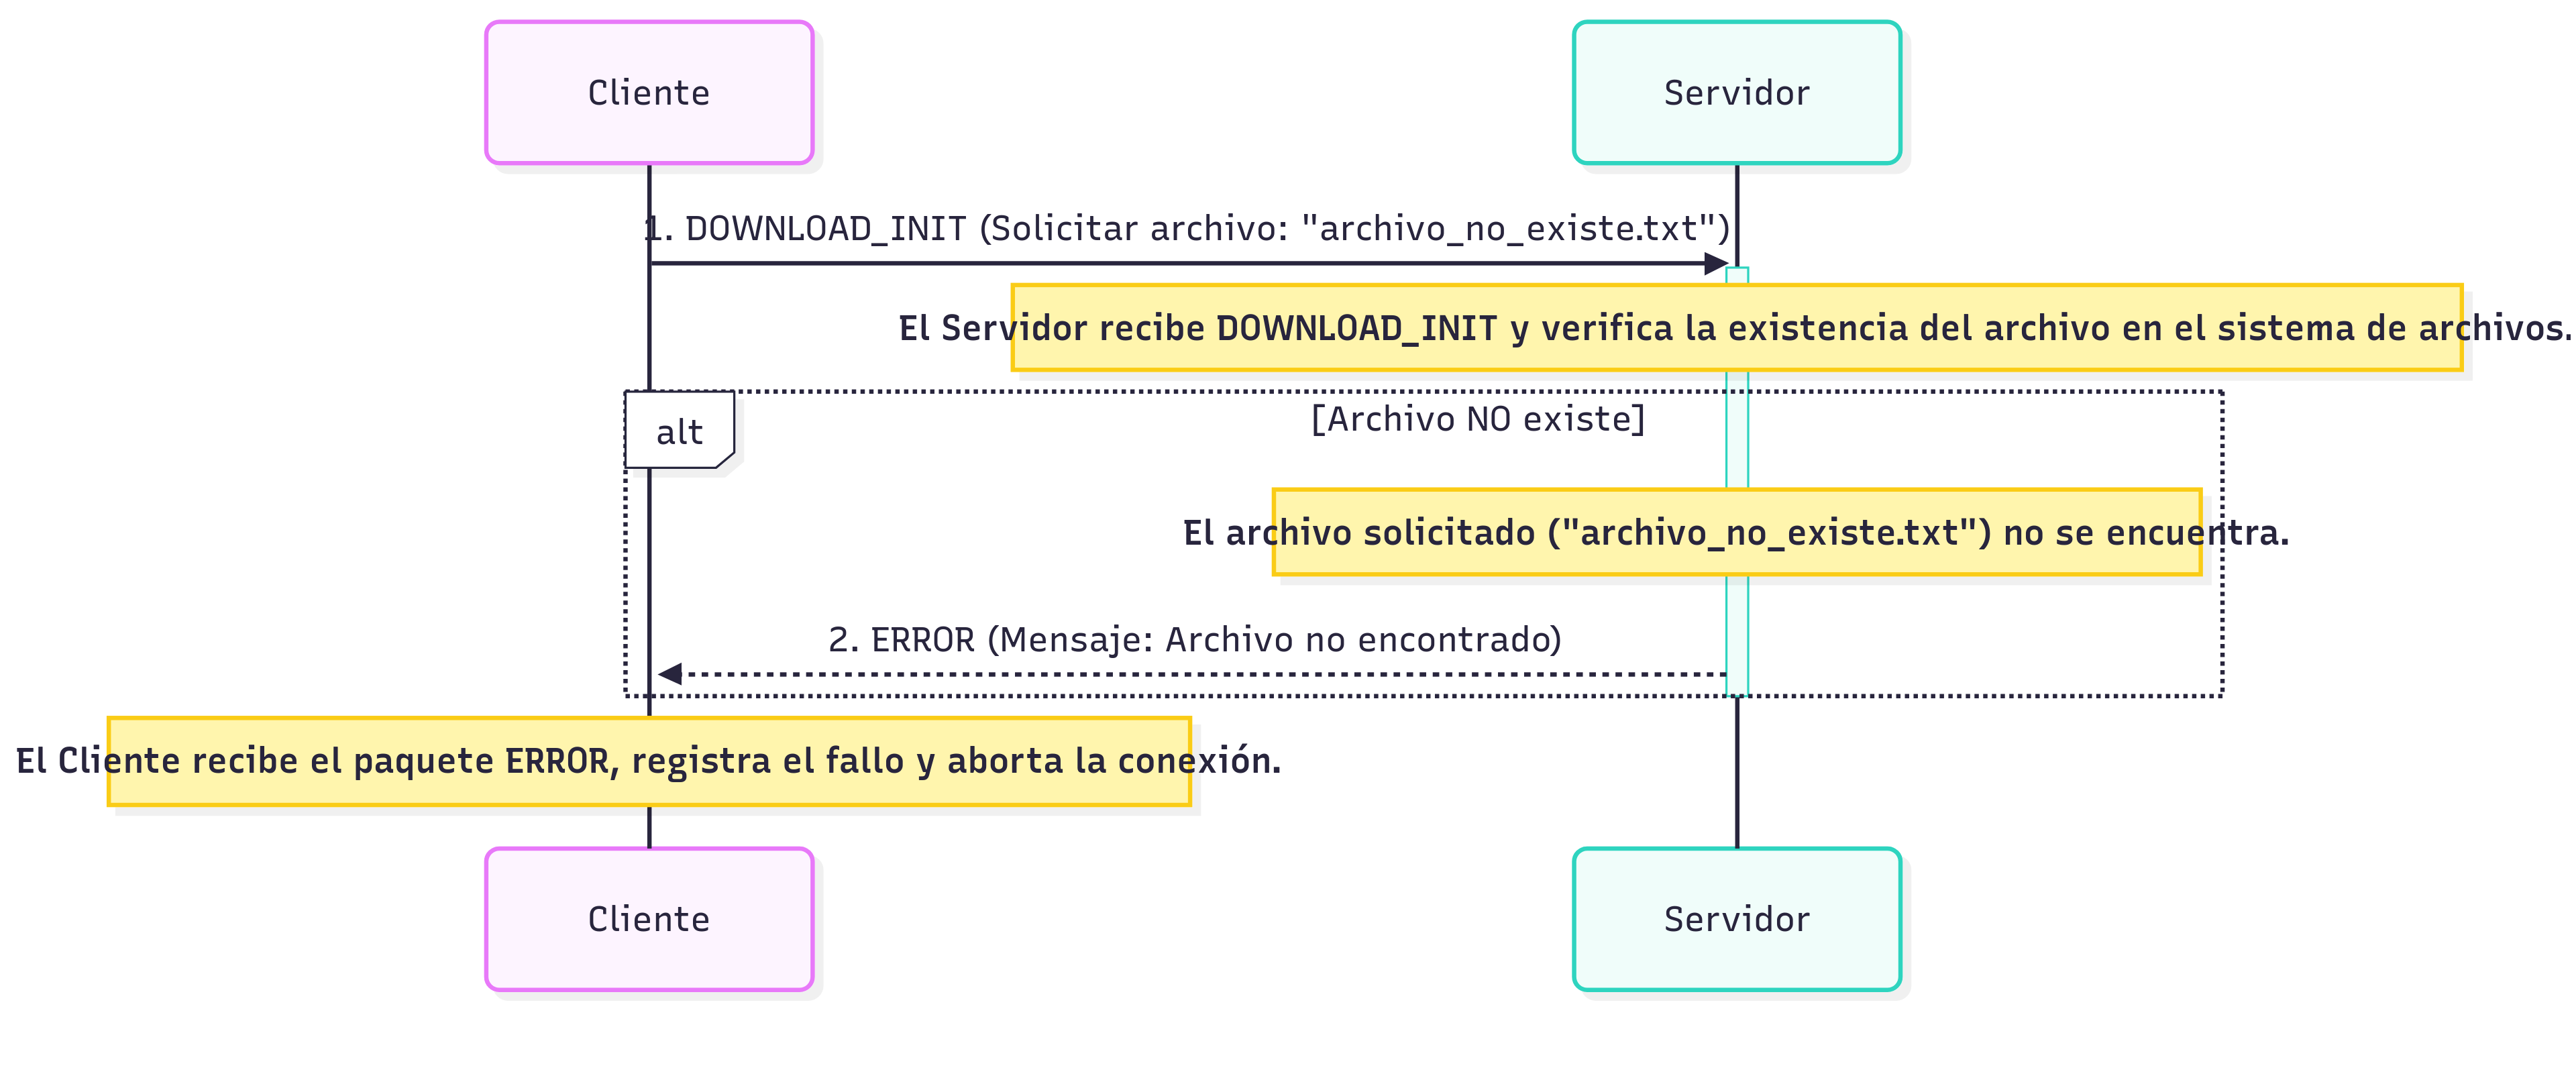
\includegraphics[width=1\linewidth]{images/diagram_sec_unexistent_file.png}
    \caption{Cierre de conexión y envio de error por solicitud de archivo inexistente.}
    \label{fig:retransmision}
\end{figure}




\subsection{Manejo de Concurrencia}

\subsubsection{Arquitectura Concurrente}
El servidor implementado es capaz de atender múltiples clientes simultáneamente sin que las transferencias interfieran entre sí.
El servidor utiliza un modelo de concurrencia basado en threads con recursos dedicados por sesión. La arquitectura se puede describir en tres niveles:

\textbf{Thread Principal (Main Thread)}

El thread principal del servidor ejecuta un loop infinito que:

\begin{enumerate}
    \item Escucha en el puerto principal (49153) solicitudes de inicio de transferencia
    \item Valida que haya capacidad disponible
    \item Crea recursos dedicados para cada nueva transferencia
    \item Delega el manejo de la transferencia a un thread dedicado
    \item Registra la sesión en el diccionario de sesiones activas
\end{enumerate}

Este diseño permite que el thread principal continúe aceptando nuevas conexiones mientras las transferencias en curso se ejecutan en paralelo.

\textbf{Threads Dedicados (Worker Threads)}

Cada transferencia corre en su propio thread con recursos completamente aislados:

\begin{itemize}
    \item \textbf{Socket UDP dedicado:} Cada sesión tiene su propio socket escuchando en un puerto dinámico único
    \item \textbf{Session ID único:} Identificador de 1-255 que no colisiona con otras sesiones activas
    \item \textbf{Estado independiente:} Variables de protocolo (ventanas, buffers) no compartidas entre threads
    \item \textbf{File descriptor:} Cada thread maneja su propio archivo sin compartir recursos de I/O
\end{itemize}

Este aislamiento garantiza que un error o problema en una transferencia no afecta a las demás.

\subsubsection{Gestión de Recursos Compartidos}

Aunque cada transferencia está mayormente aislada, existen algunos recursos compartidos que requieren sincronización cuidadosa:

\textbf{Diccionario de Sesiones Activas}

El servidor mantiene un diccionario global de todas las sesiones activas, que contiene para cada sesión:

\begin{itemize}
    \item \texttt{session\_id}: Identificador único (1-255)
    \item \texttt{dedicated\_port}: Puerto UDP asignado
    \item \texttt{thread}: Referencia al thread worker
    \item \texttt{dedicated\_socket}: Socket UDP dedicado
    \item \texttt{client\_addr}: Dirección IP y puerto del cliente
    \item \texttt{created\_at}: Timestamp de creación
\end{itemize}

Para garantizar consistencia, todas las operaciones sobre este diccionario están protegidas por un lock (\texttt{sessions\_lock}). Las operaciones sincronizadas incluyen:

\begin{itemize}
    \item Agregar nueva sesión
    \item Remover sesión completada
    \item Verificar cantidad de sesiones activas
    \item Generar session ID único
\end{itemize}

\subsubsection{Puertos Dedicados}

Cada transferencia obtiene su propio puerto UDP, lo que proporciona aislamiento a nivel de socket del sistema operativo.

\textbf{Asignación Dinámica de Puertos}

El servidor crea un socket UDP y lo vincula al puerto 0, lo que indica al sistema operativo que asigne automáticamente un puerto disponible del rango de puertos dinámicos (típicamente 49152-65535). Este mecanismo tiene varias ventajas:

\begin{enumerate}
    \item \textbf{Aislamiento completo:} Los paquetes de diferentes transferencias nunca se mezclan, ya que cada una tiene su propio socket

    \item \textbf{Sin multiplexación:} No hay necesidad de demultiplexar paquetes por session\_id en el socket principal, simplificando la lógica

    \item \textbf{Simplicidad:} Cada thread puede ejecutar \texttt{recvfrom()} sin condiciones de carrera ni coordinación con otros threads

    \item \textbf{Escalabilidad:} El sistema operativo maneja eficientemente la distribución de puertos y el enrutamiento de paquetes

    \item \textbf{Robustez:} Si un socket falla o se bloquea, no afecta a los demás
\end{enumerate}

\subsubsection{Control de Capacidad}

El servidor implementa un límite configurable de transferencias concurrentes para prevenir agotamiento de recursos del sistema.

Antes de aceptar una nueva transferencia, el servidor verifica que el número de sesiones activas no supere el máximo configurado (10 por defecto). Si el servidor está a capacidad:

\begin{enumerate}
    \item Se registra una advertencia en los logs
    \item Se envía un paquete ERROR al cliente con el mensaje ``Server at capacity, try again later''
    \item Se rechaza la conexión sin crear recursos
    \item El cliente puede reintentar más tarde
\end{enumerate}

\subsubsection{Flujo Completo de una Sesión Concurrente}

A continuación se describe el ciclo de vida completo de una sesión en el servidor concurrente:

\begin{figure}[H]
\centering
\small
\begin{minipage}{0.9\textwidth}
\begin{verbatim}
1. Cliente envia UPLOAD_INIT/DOWNLOAD_INIT al puerto 49153
   |
   +---> Thread Principal recibe solicitud
   |    |
   |    +---> Adquiere lock sobre sessions_lock
   |    +---> Verifica capacidad (< 10 sesiones)
   |    +---> Libera lock
   |
   +---> Si capacidad disponible:
   |    |
   |    +---> Genera session_id unico (con lock)
   |    +---> Crea socket dedicado en puerto N
   |    +---> Envia ACCEPT(session_id, puerto N)
   |    |
   |    +---> Crea thread dedicado T
   |    +---> Registra sesion en active_sessions (con lock)
   |    +---> Inicia thread: T.start()
   |
   +---> Si capacidad completa:
        +---> Envia ERROR("Server at capacity")

2. Thread Dedicado T ejecuta:
   |
   +---> Espera ACCEPT_ACK en socket dedicado
   +---> Crea instancia de protocolo (Stop&Wait o Selective Repeat)
   +---> Ejecuta transferencia (bloqueante solo para este thread)
   +---> Guarda archivo en disco
   |
   +---> Finally (siempre ejecuta):
        +---> Adquiere lock sobre sessions_lock
        +---> Elimina sesion de active_sessions
        +---> Libera lock
        +---> Cierra socket dedicado

3. Thread Principal continua:
   +---> Loop: Espera proxima solicitud (no bloqueado por T)
\end{verbatim}
\end{minipage}
\caption{Ciclo de vida de una sesión concurrente}
\end{figure}




% PENDIENTE AGREGAR SECCIONES QUE EXPLIQUEN EN CONCRETO LA IMPLE DEL STOP & WAIT Y EL SELECTIVE REPEAT

\subsection{Stop \& Wait}
\subsection{Selective Repeat}
